\documentclass[10pt,a4paper]{article}
\usepackage[utf8]{inputenc}
\usepackage[spanish,es-noshorthands]{babel}
\usepackage{amsmath}
\usepackage{amsfonts}
\usepackage{amssymb}
\usepackage{graphicx}
\author{Germán Avendaño Ramírez}
\title{Ejercicio}
\begin{document}
\maketitle
\section*{3.4.1 Ejercicios}
\begin{enumerate}
\item[f] $2\sqrt[3]{x}-\sqrt[3]{x^2}+8=0$
\end{enumerate}
\subsection*{Soluci\'on}
Expreso lo mismo usando exponentes:
\[2x^{1/3}-x^{2/3}+8=0\]
Ahora ordeno de mayor a menor exponente, para asimilarla a una cuadrática:
\begin{align*}
-x^{2/3}+2x^{1/3}+8&=0 &\\
x^{2/3}-2x^{1/3}-8&=0 & \mbox{Multiplicando por $-1$ la ecuación}\\
(x^{1/3}-4)(x^{1/3}+2)&=0 & \mbox{se buscan dos números que sumados den $-2$ y multiplicados $-8$}
\end{align*}
Luego entonces se tiene que:
\[x^{1/3}-4=0 \qquad \mbox{ó} \qquad x^{1/3}+2=0\]
Por tanto
\begin{align*}
x^{1/3}-4=&0\\
x^{1/3}=&4\\
x=&4^{3}\\
x=&64
\end{align*}
ó
\begin{align*}
x^{1/3}+2&=0\\
x^{1/3}&=-2\\
x&=-2^{3}\\
x&=-8
\end{align*}

Por tanto las dos ráices son --8 y 64. 
Esto se corrobora con la gráfica de la función $f(x)=2\sqrt[3]{x}-\sqrt[3]{x^{2}}+8$
\begin{center}
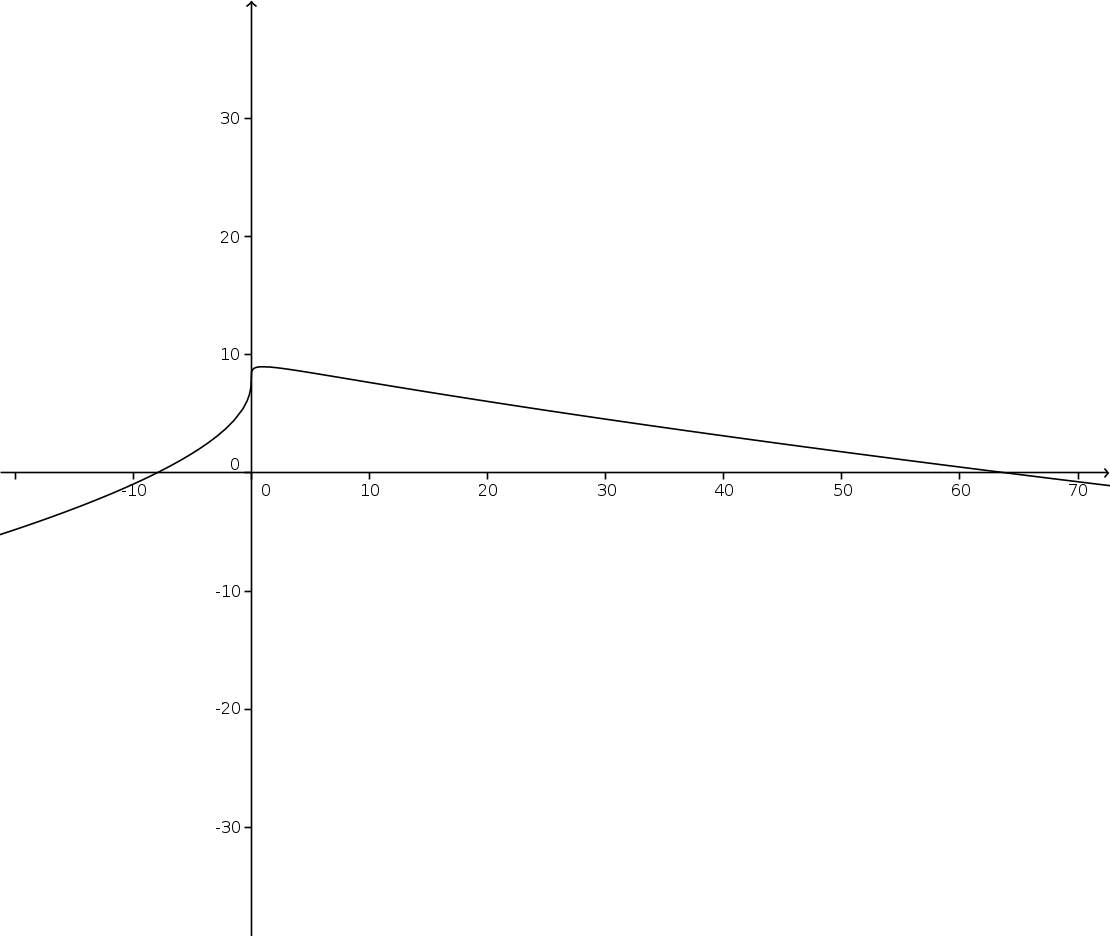
\includegraphics[scale=1]{Images/funcion.png} 
\end{center}
\end{document}